\chapter{ADVANCE SOLUTION}
\label{chap:adva}

\section{Lemmas That Help to Prune}

Baseline solution basically is just a brute force method. Now we introduce some 
lemmas that prunes and accelerates the baseline solution.


{\bfseries Definition 4.} A product $p$ dominates another product $q$ 
if and only if $\forall i \in [1, d]$, the $i_{th}$ dimension $p[i] \geq q[i]$ and $\exists$ $i \in [1,d]$, the $i_{th}$ dimension $p[i]>q[i]$.

{\bfseries Lemma 1.} If  $\forall q$ that $C(q)<B, \exists p$ that $C(p)=B$ and $p$ dominates $q$, then there must be at least one optimal solution on $C(p)=B$.

Because for most of the constraint $C(p)<B$ is bounded by $C(p)=B$ and as for our defined 
constraint $\Sigma_{i=1}^d p[i] \leq B$ satisfies condition of Lemma 1, in 
experiments we only need to consider region $C(p)=B$ as our candidate space which is also the root node of $CellTree$.

On the base of Lemma 1 that only consider $C(p)=B$, which also means only $h_i$ will divide space 
$C(p)=B$ would affect where the optimal solutions are, we define Lemma 2.

{\bfseries Lemma 2.} Ignore the users $w$ such that $w\cdot p=S_k$ doesn't intersect with constraint $C(p)=B$ won't affect the $kCRM$ result.

\begin{figure}[hbt!]
  \centering
  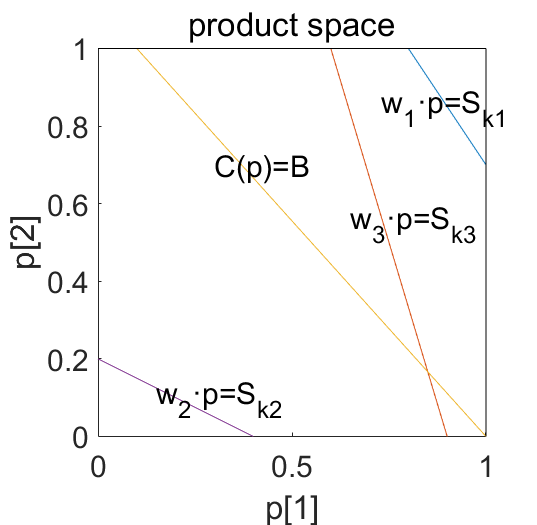
\includegraphics[width=.5\linewidth]{the_intersect.png}
  \caption{User Intersect With constraint}
  \label{explain_intersect}
\end{figure}

As shown in Figure \ref{explain_intersect}, if we decide to choose the new product
 from $C(p)=B$, we can see that $h_1$ also divides the product space into 2
  halfspaces, but all the products on $C(p)=B$ are in the “-” halfspace, 
  which means all of them can not cover $w_1$. 
  Different from $w_1$, the products that on $C(p)=B$ all can cover $w_2$. 
  From this observation, we can move out all the users $w$ such that 
  $w_i \cdot p=S_{ik}$ doesn't intersect with $C(p)=B$.


 
{\bfseries Definition 5.} The negative space count for a $CellTree$ node is the 
negative spaces from this node to root node traversing by ancestor node one by one.

Take Figure \ref{cell_tree_nodes} as an example, the negative space count
\begin{enumerate}
\item For cell $c_4$ is 1 because of $h_2^-$,
\item For cell $c_5$ is 1 because of $h_1^-$, 
\item For cell $c_6$ is 2 because of $h_1^-$ and $h_2^-$.
\end{enumerate}

{\bfseries Lemma 3.} If the cover count of optimal solution in $kCRM$ is at least 
$\beta $ and $card(W)=n$, then all the 
nodes with more than $n-\beta $  can't become the optimal solution and they can 
be pruned.

Lemma 3 means that if we can judge there is no solution in a space can become 
optimal solution because them can't cover at least $\beta$ users, then we can 
prune this space. Take Figure \ref{cell_tree_nodes} as example, if $\beta=2$ 
which means the optimal solution should at least cover 2 users 
and $W=\{w_1, w_2, w_3\}$, then the nodes $c_3$, $c_4$, $c_5$ can be pruned 
because they can never cover at least 2 users even after the insertion of 
$h_3$. Actually, $\beta$ is the lower bound of optimal solution.

{\bfseries Definition 6.} Pruning number $\alpha $ is defined as $\alpha = n-\beta $ 
which based on Lemma 3.

Pruning number $\alpha$ means that if a node's negative space count exceeds 
$\alpha$, than it is safe to prune this node.

\section{Get Pruning Number}
Based on Lemma 3, to find a proper $\beta$, we simply uniformly generate new 
products 
in candidate space and then find the maximal cover count of them.
The procedure is:
\begin{enumerate}
\item Uniformly generate new products $P'=$\{$p_{1}', ..., p_{y}'$\} on $C(p')=B$.
\item Calculate cover count of each of $P'$.
\item Find the maximal cover count of $P'$ as $\beta$
\item Pruning number $\alpha=card(W)-\beta$ 
\end{enumerate}



\section{Insertion Order of Users}

{\bfseries Definition 7.} Maximal likely cover count of a user means  
the maximal cover count of the sampled products that cover this user.

As mentioned in Lemma 3, we prune the cell nodes that with more that $\alpha$ 
negative halfspaces. 
To be earlier prune the nodes that itself and its sub-tree leaf nodes can't be 
optimal solution,
we can firstly insert the halfspace that its positive halfspace not likely be 
the component of optimal solutions.
Our method to determinate the insertion order of halfspace is by the maximal 
likely cover count of users (we write CoverCount in short as CC):

\begin{enumerate}
  \item Initialize the cover count of each user as 0.
  \item Uniformly generate new products $P'=$\{$p_{1}', ..., p_{y}'$\} on $C(p')=B$.
  \item for $p'$ in $P'$ 
  \begin{enumerate}
    \item $W'$ is the user set covered by $p$
    \item $p'.CC=card(W')$
    \item for $w'$ in $W'$
    \begin{enumerate}
      \item $w'.CC=max(w'.CC, p.CC)$
    \end{enumerate}
  \end{enumerate}
  \item update $W=AscendingSortByCC(W)$
  \item return $W$
\end{enumerate}


{\bfseries Lemma 4.} Insert users by the order of their maximal likely cover counts in ascending.

The assumption that proposes Lemma 4 is that we don't want those users positive 
halfspaces $h_i^i$
hide with the user positive halfspaces can be part of optimal because that would make 
us use $\alpha$ to prune nodes quit late for it has generate many nodes can't be
part of optimal solutions. 




\section{Summary of Lemmas}
\begin{enumerate}
    \item Lemma 1 prunes the candidate space from $C(p) \leq B$ to $C(p)=B$.
    \item Lemma 2 moves out the users $w$ that $w\cdot p=S_k$ doesn't intersect with $C(p)=B$
    \item Lemma 3 state that in the process of $CellTree$ we can prune the nodes whose negative space count is more than pruning number $\alpha$. 
    \item Lemma 4 introduces a heuristic trick that forces pruning some nodes using
    Lemma 3.   
  \end{enumerate}

\section{Advance Solution}
The main procedure for advance solution in short is:
\begin{enumerate}
  \item Remove users covered by $P$.
  \item Remove users by Lemma 2.
  \item Apply Lemma 4 change the insertion order of users' halfspace.
  \item Apply Lemma 1 on root node of $CellTree$.
  \item Apply Lemma 3 prune nodes when doing $CellTree$ insertion.
\end{enumerate}
For more details:
\begin{enumerate}
\item Calculate the top-$k$ score $S_{ik}$ for each $w_i\in W$.
\item Find all the $w_i\in W$ that $P$ covers, mark their set as $W^*$.
\item Update $W=W-W^*$.
\item Find all the $w_i\in W$ that $w_i\cdot p=S_{ik}$ doesn't intersect with $C(p)=B$, mark their set as $W^{**}$.
\item Update $W=W-W^{**}$.
\item Generate new products on candidate space and find their maximal cover count as $\beta$
\item Let pruning number $\alpha =card(W)-\beta $
\item Update candidate space from $C(p) \leq B$ to the part of $C(p)=B$.
\item Chnage order of users $W$ as defined in Lemma 4
\item For $w_i \in W$,
try to insert $h_i$ for existing $CellTree$ using depth first search.
\begin{enumerate}
\item If the current node is marked as pruned, return.
\item Else if the node is in $h_i^-$, increase its negative space count by 1.
\begin{enumerate}
  \item If the node's negative space count exceeds $\alpha$ mark it as pruned.
  \item Increase its sub-tree nodes' negative space count by 1.
\end{enumerate} 
\item Else if the node is in $h_i^+$, increase its child nodes' and its cover count by 1.
\item Else if there is no child nodes of current node, generate two child nodes as 
      $h_i^-$ and $h_i^+$, return. 
\item Else if two child nodes marked as pruned, the current node is also marked as pruned
\item Else traverse to its child nodes.
\end{enumerate}
\item Return the node with maximal cover count.
\end{enumerate}

\section{Time Complexity}
As memtioned in Section \ref{baseline_tc}, the baseline's time complexity is $O(n^d)$.
For advance solution, we reduce the candidate space from $C(p)\leq B$ to $C(p)=B$, 
which actually reduces our time complexity to $O(n^{d-1})$ because the candidate space
reduces by 1 dimension and the insertion halfspace reduces by 1 dimension together.
Besides, we remove the users that doesn't intersect with $C(p)=B$. Actually, some of these users
may related to the optimal solution, for example their halfspace may enclose
the optimal solution region but since we give up all the candidate space of 
$C(p)<B$ they then just look unrelated to the optimal solution. In fact, if we want
an optimal solution with the lower cost we need those users that $h_i^-$ are totally
cover by $C(p)\leq B$. Back to the thesis of this section, the $n$ in $O(n^{d-1})$
reduces users quit a lot. We use $n_{new}$ to represented the cardinality of 
user data after removing the user by Lemma 3, then our time complexity is $O(n_{new}^{d-1})$.

